\documentclass[10pt,a4paper]{article}

% Language setting
\usepackage[british]{babel}

% Set page size and margins
\usepackage[a4paper,top=2cm,bottom=2cm,left=2.5cm,right=2.5cm,marginparwidth=1.75cm]{geometry}

\usepackage[style=ieee, backend=biber]{biblatex} % IEEE style citations using biblatex
\addbibresource{references.bib} % Your .bib file


\usepackage{amsmath}
\usepackage{graphicx}
\usepackage[colorlinks=true, allcolors=blue]{hyperref}
\usepackage{hyperref}
\usepackage{orcidlink}
\usepackage[title]{appendix}
\usepackage{mathrsfs}
\usepackage{amsfonts}
\usepackage{booktabs} % For \toprule, \midrule, \botrule
\usepackage{caption}  % For \caption
\usepackage{threeparttable} % For table footnotes
\usepackage{algorithm}
\usepackage{algorithmicx}
\usepackage{algpseudocode}
\usepackage{listings}
\usepackage{enumitem}
\usepackage{chngcntr}
\usepackage{booktabs}
\usepackage{lipsum}
\usepackage{subcaption}
\usepackage{authblk}
\usepackage[T1]{fontenc}    % Font encoding
\usepackage{csquotes}       % Include csquotes
\usepackage{diagbox}


% Customize line spacing
\usepackage{setspace}
\onehalfspacing % 1.5 line spacing

% Redefine section and subsection numbering format
\usepackage{titlesec}
\titleformat{\section} % Redefine section numbering format
  {\normalfont\Large\bfseries}{\thesection.}{1em}{}
  
% Customize line numbering format to right-align line numbers
\usepackage{lineno} % Add the lineno package
\renewcommand\linenumberfont{\normalfont\scriptsize\sffamily\color{blue}}
\rightlinenumbers % Right-align line numbers

\linenumbers % Enable line numbering

% Change the position of the table caption above the table
\usepackage{float}   % for customizing caption position
\usepackage{caption} % for customizing caption format
\captionsetup[table]{position=top} % caption position for tables

% Define the unnumbered list
\makeatletter
\newenvironment{unlist}{%
  \begin{list}{}{%
    \setlength{\labelwidth}{0pt}%
    \setlength{\labelsep}{0pt}%
    \setlength{\leftmargin}{2em}%
    \setlength{\itemindent}{-2em}%
    \setlength{\topsep}{\medskipamount}%
    \setlength{\itemsep}{3pt}%
  }%
}{%
  \end{list}%
}
\makeatother

% Suppress the warning about \@parboxrestore
\pdfsuppresswarningpagegroup=1


%-------------------------------------------
% Paper Head
%-------------------------------------------
\title{[Proposal title]}

\author{
    First Last (\texttt{OsirisID}), 
    First Last (\texttt{OsirisID})
}

\date{}  % Remove date

\begin{document}
\maketitle

\textbf{Overall comment:}
A proposal needs to show how your work fits into what is already known about the topic and what it will contribute to the literature. In addition, it should specify the research question(s) that the research will answer, establishing its significance, and the implications of the answer.

\textbf{Key points:}
\begin{itemize}
    \item Max. 6 pages excluding figures, tables, and references
    \item Adhere to the template as shown here
    \item Keep sentences short and concise
    \item Explain/justify all choices via a reference, formal proof, empirical proof, or solid reasoning
    \item Use IEEE citation style
\end{itemize}

%-------------------------------------------
% Paper Body
%-------------------------------------------
\section{Introduction}\label{sec:introduction}
The introduction is your chance to grab the reader's attention and set the stage for your research. It should spark interest and provide enough context for the audience to understand the text ahead.

Begin by introducing a broad issue that resonates with your target audience. For example, if you're researching the impact of social media on mental health in teenagers, you could start with a statistic about overall social media usage among teens. Gradually narrow your focus by highlighting a specific concern, such as the potential link between increased social media use and anxiety symptoms.

Throughout your introduction, use relevant, credible, and up-to-date references to support your claims. This demonstrates your understanding of the field and strengthens the foundation of your research proposal.

\section{Related work}\label{sec:relatedwork}
In most cases, you are not the first to study your topic in science. The related work section allows you to present and discuss previous works that relate to your idea. Note that this should not merely be a list of previous works and what they did. Try to distill, describe, and discuss overarching themes in methods and results. This section should be heavily cited. 

Often, there will not be many papers that pursue your exact idea and methodology. Hence, the related work section is often split up into different sections where each section focuses on a specific aspect of your proposed research idea. For example, when researching dementia diagnosis in elderly people using remote healthcare solutions, one section could summarize the works on dementia diagnosis, while another could focus on the use of wearables in the elderly patient population. 

As you discuss previous studies, don't shy away from critical analysis. However, make sure to support your criticism well. Highlight the strengths and limitations of existing research, and explain how your study aims to address any gaps in knowledge. 

\section{Research question}\label{sec:researchquestion}
After discussing the context of your topic and other works related, you define the main research question and possible sub research questions. The research question is the heart of your proposal. It's the precise question you aim to answer through your study. Here are some key points to consider:

\begin{itemize}
    \item Formulate a clear and concise research question that leaves no room for ambiguity. Avoid overly broad questions that lack a defined direction.
    \item Ensure your research question aligns with the chosen statistical analysis methods. Remember, your study should involve at least two independent variables and two dependent variables, or utilize a within-subjects design.
\end{itemize}

\section{Methodology}\label{sec:methods}
In this section you describe what, why, and how you want to find answers to your research question(s). In a proposal, this section needs to convince that the data and methodology chosen are adequate to answer the research question. This section is also the place to explain how you plan to extract features from the raw data streams. For example, how to extract tonic level from electrodermal activity (i.e., sweat gland activity) or how to aggregate one's heart rate over the span of a night. Your explanations should be clear and comprehensive enough for someone else to replicate your study. 

Be sure to justify your choices at each step. Explain why you've selected a specific data source, experimental design, or analytical technique. Connect these choices back to your research question and the type of data you'll be working with.

\subsection{Data (if using existing dataset)}
Name the dataset you will use and its origin. Describe its contents, focus, the type of data, etc. Explain why this dataset is relevant to your research question. 

\subsection{Experimental design (if collecting own data)}
If you decided to collect your own data, please give a detailed account on how you plan to obtain the data. What is the target population, what is the experimental protocol, what quantitative research methods are you planning to use? Also, specify the minimal number of participants you need per class and think about how you balance your dataset in terms of gender, age, and other demographics. Additionally, come up with a fall-back plan in the form of an existing dataset that allows you to still conduct your statistical analysis if things go sideways. For example, you did not find enough participants or the quality of the measured data is too low, resulting in many missing data points. 

\subsection{Preprocessing and feature extraction}
Specify which variables/features you intend to analyze and use to answer your research question and justify these choices. Describe how you intend to extract these features from your data. Describe the entire preprocessing and feature extraction pipeline as detailed as possible. By thinking about your processing pipeline beforehand, you'll save a considerable amount of time in the second phase of the project.
If you collect your own data, this section would likely only describe preprocessing.

\subsection{Analysis}
Name the specific statistical tests or analyses you will apply (see flowchart presented during Lecture: Preliminaries/overview, ANOVA (1/3) (one-way)). Justify the choices based on your research question and type of data and analysis. Describe your dependent and independent variables. 

\textbf{Note:}
\begin{itemize}
    \item Statistical analysis should include >1 independent and >1 dependent variable or a within subjects design (both are also fine). 
    \item Suggest a post-hoc analysis or supplementary analysis including an appropriate type of regression analysis or a well-justified alternative
\end{itemize}

\section{Timeline}
Presenting an initial timeline forces you to think about potential time-consuming steps in your research beforehand. Typically, a Gantt-chart is used for visualization (see~Figure~\ref{fig:gantt})

\begin{figure}[hbtp]
    \centering
    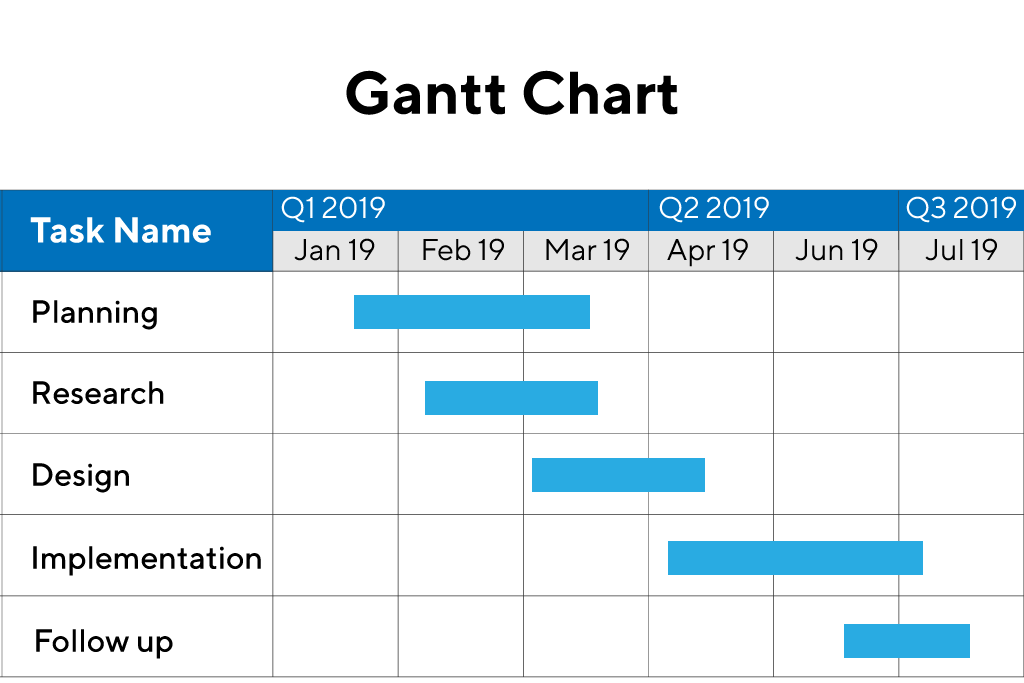
\includegraphics[width=0.7\textwidth]{figures/Gantt-chart.png}
    \caption{Example of a Gantt-chart that shows the expected timeline of your research.}
    \label{fig:gantt}
\end{figure}

\section{Contributions}
Conclude your proposal by restating the implications of your work and your contributions to science and society. Your work might strengthen our knowledge about a specific topic or creates a basis for future research. Use this section to explain and emphasize these aspects of your proposal to convince the reader of your research idea one last time.

% Print bibliography
\printbibliography

\newpage
\begin{appendices}

%--- Section ---%
\section{How to Include Equations}\label{sec4}

Equations in \LaTeX{} can either be inline or set as display equations. For
inline equations use the \verb+$...$+ commands. Eg: the equation
$H\psi = E \psi$ is written via the command \verb+$H \psi = E \psi$+.

For display equations (with auto generated equation numbers)
one can use the equation or eqnarray environments:
\begin{equation}
\|\tilde{X}(k)\|^2 \leq\frac{\sum\limits_{i=1}^{p}\left\|\tilde{Y}_i(k)\right\|^2+\sum\limits_{j=1}^{q}\left\|\tilde{Z}_j(k)\right\|^2 }{p+q},
\label{eq1}
\end{equation}
where
\begin{align}
D_\mu &=  \partial_\mu - ig \frac{\lambda^a}{2} A^a_\mu \nonumber \\
F^a_{\mu\nu} &= \partial_\mu A^a_\nu - \partial_\nu A^a_\mu + g f^{abc} A^b_\mu A^a_\nu
\label{eq2}
\end{align}
Notice the use of \verb+\nonumber+ in the align environment at the end
of each line, except the last, so as not to produce equation numbers on
lines where no equation numbers are required. The \verb+\label{}+ command
should only be used at the last line of an align environment where
\verb+\nonumber+ is not used.
\begin{equation}
Y_\infty = \left( \frac{m}{\textrm{GeV}} \right)^{-3}
    \left[ 1 + \frac{3 \ln(m/\textrm{GeV})}{15}
    + \frac{\ln(c_2/5)}{15} \right]
\label{eq3}
\end{equation}
The class file also supports the use of \verb+\mathbb{}+, \verb+\mathscr{}+ and
\verb+\mathcal{}+ commands. As such \verb+\mathbb{R}+, \verb+\mathscr{R}+
and \verb+\mathcal{R}+ produces $\mathbb{R}$, $\mathscr{R}$ and $\mathcal{R}$
respectively 
%(refer Subsubsection~\ref{subsubsec3}).

Equations must be provided as editable text, either in a Word or LaTeX source file. They should be numbered consecutively through the manuscript as shown in Equations \ref{eq1}, \ref{eq2} and \ref{eq3}. In APA style, when discussing numbered equations in the text, write out the word “Equation” and give the number. For example, you would write “see Equation \ref{eq1}.”
Use no punctuation after the equation if it appears at the end of a sentence; however, it is permissible (and may even be necessary) to place some form of punctuation after it (a comma or semi-colon, for example) if it appears in the middle of the sentence and is followed by text. In any case, maintain the coherence of all sentences with equations in them.


%--- Section ---%
\section{Tables}\label{sec5}

Use the table and tabular environments for basic tables --- see Tables~\ref{tab1} and \ref{tab2}, for example. Table \ref{tab1} is an sample figure including table footnotes. For more information, please see this help article on \href{https://www.overleaf.com/learn/latex/tables}{tables}. The general table style should only include horizontal rules at the top, after the header row, and at the bottom of the table. Tablenotes can be used to note small details otherwise too minor to be put in the main text.

\begin{table}[!ht]
\caption{Sample table with footnotes\label{tab1}}
\begin{threeparttable}
\begin{tabular*}{\columnwidth}{@{\extracolsep\fill}llll@{\extracolsep\fill}}
\toprule
column 1 & column 2 & column 3 & column 4\\
\midrule
row 1 & data 1 & data 2 & data 3 \\
row 2 & data 4 & data 5\tnote{1} & data 6 \\
row 3 & data 7 & data 8 & data 9\tnote{2} \\
\bottomrule
\end{tabular*}
\begin{tablenotes}
\item Source: This is an example of table footnote. This is an example of table footnote. This is an example of table footnote. This is an example of table footnote. This is an example of table footnote.
\item[1] Example for a first table footnote.
\item[2] Example for a second table footnote.
\end{tablenotes}
\end{threeparttable}
\end{table}

\begin{table*}[!ht]
\caption{Example of a lengthy table which is set to full textwidth.\label{tab2}}
\tabcolsep=0pt
\begin{threeparttable}
\begin{tabular*}{\textwidth}{@{\extracolsep{\fill}}lcccccc@{\extracolsep{\fill}}}
\toprule
& \multicolumn{3}{c}{Element 1\tnote{1}} & \multicolumn{3}{c}{Element 2\tnote{2}} \\
\cmidrule(lr){2-4}\cmidrule(lr){5-7}
Project & Energy & $\sigma_{\mathrm{calc}}$ & $\sigma_{\mathrm{expt}}$ & Energy & $\sigma_{\mathrm{calc}}$ & $\sigma_{\mathrm{expt}}$ \\
\midrule
Element 3 & 990 A & 1168 & $1547\pm12$ & 780 A & 1166 & $1239\pm100$ \\
Element 4 & 500 A & 961 & $922\pm10$ & 900 A & 1268 & $1092\pm40$ \\
\bottomrule
\end{tabular*}
\begin{tablenotes}
\item Note: This is an example of table footnote this is an example of table footnote this is an example of table footnote this is an example of~table footnote this is an example of table footnote.
\item[1] Example for a first table footnote.
\item[2] Example for a second table footnote.
\end{tablenotes}
\end{threeparttable}
\end{table*}


%--- Section ---%
\section{Figures}\label{sec6}

First you have to upload the image file from your computer using the upload link in the file-tree menu. Then use the includegraphics command to include it in your document. Use the figure environment and the caption command to add a number and a caption to your figure. See the code for Figure \ref{fig:frog} in this section for an example. As shown in Figures \ref{fig:frog} and \ref{fig:multi_figs}, the images should be single-page documents. 

Note that your figure will automatically be placed in the most appropriate place for it, given the surrounding text and taking into account other figures or tables that may be close by. You can find out more about adding images to your documents in this help article on \href{https://www.overleaf.com/learn/how-to/Including_images_on_Overleaf}{including images on Overleaf}.

\begin{figure}[!ht]
\centering
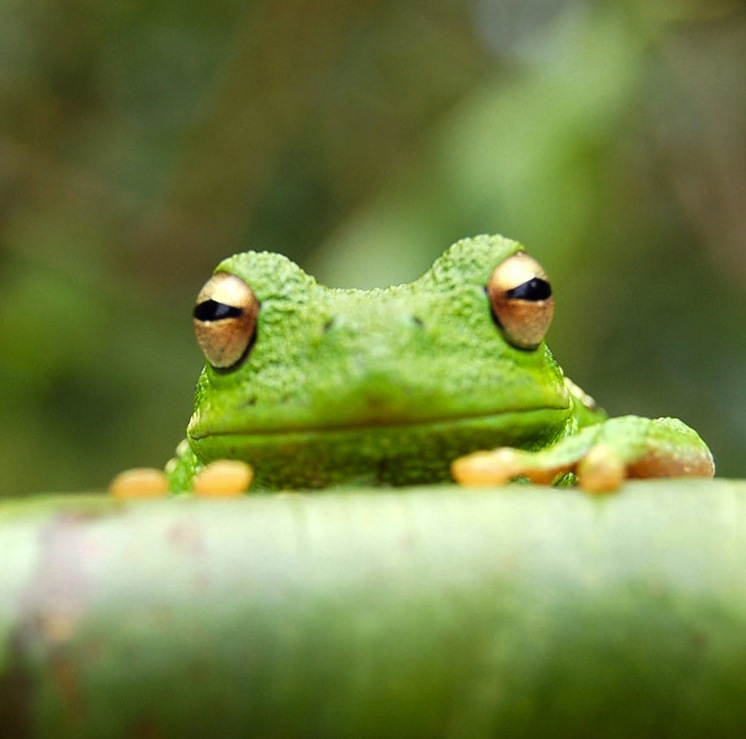
\includegraphics[width=0.4\linewidth]{figures/frog.jpg}
\caption{\label{fig:frog}This frog was uploaded via the file-tree menu.}
\end{figure}

\subsection{More information about figures}

As per display \LaTeX\ standards one has to use eps images for \verb+latex+ compilation and \verb+pdf/jpg/png+ images for
\verb+pdflatex+ compilation. This is one of the major differences between \verb+latex+
and \verb+pdflatex+. The images should be single-page documents. The command for inserting images
for \verb+latex+ and \verb+pdflatex+ can be generalized. The package used to insert images in \verb+latex/pdflatex+ is the
graphicx package. Figures can be inserted via the normal figure environment as shown in the below example:


\begin{figure}[!ht]
    \begin{subfigure}{0.3\textwidth}
        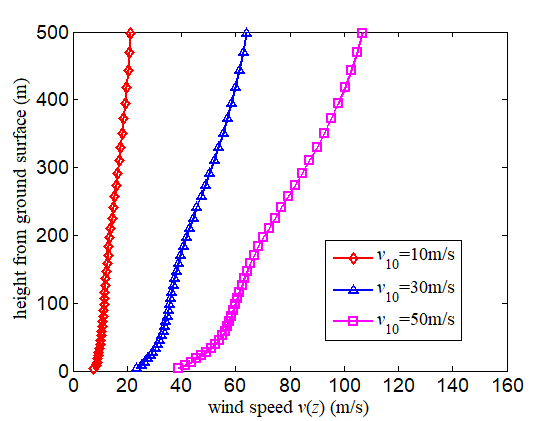
\includegraphics[width=\linewidth]{figures/fig_a.png}
        \caption{}
    \end{subfigure}
    \hfill
    \begin{subfigure}{0.3\textwidth}
        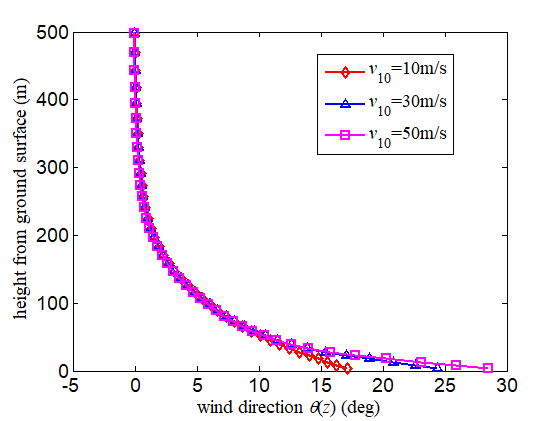
\includegraphics[width=\linewidth]{figures/fig_b.png}
        \caption{}
    \end{subfigure}
    \hfill
    \begin{subfigure}{0.3\textwidth}
        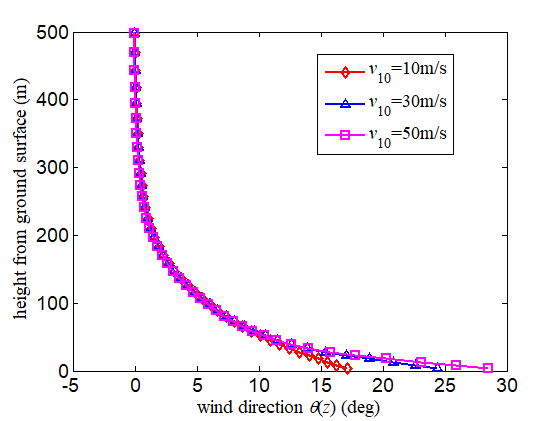
\includegraphics[width=\linewidth]{figures/fig_c.png}
        \caption{}
    \end{subfigure}
    \caption{Overall caption for the three figures: (a) caption for figure a, (b) caption for figure b, and (c) caption for figure c.}
    \label{fig:multi_figs}
\end{figure}


\begin{verbatim}
\begin{figure}[h]
        \centering\includegraphics{<eps-file>}
        \caption{<figure-caption>}
        \label{<figure-label>}
\end{figure}
\end{verbatim}


%--- Section ---%
\section{How to Include Algorithms, Program Codes, and Listings}\label{sec8}
Packages \verb+algorithm+, \verb+algorithmicx+, and \verb+algpseudocode+ are used for setting algorithms in latex.
For this, one has to use the below format:

\begin{verbatim}
\begin{algorithm}
\caption{<alg-caption>}\label{<alg-label>}
\begin{algorithmic}[1]
. . .
\end{algorithmic}
\end{algorithm}
\end{verbatim}

You may need to refer to the above-listed package documentation for more details before setting an \verb+algorithm+ environment.
To set program codes, one has to use the \verb+program+ package. We need to use the \verb+\begin{program}+ \verb+...+
\verb+\end{program}+ environment to set program codes.

\begin{algorithm}[!ht]
\caption{Calculate $y = x^n$}\label{algo1}
\begin{algorithmic}[1]
\Require $n \geq 0 \vee x \neq 0$
\Ensure $y = x^n$
\State $y \Leftarrow 1$
\If{$n < 0$}
        \State $X \Leftarrow 1 / x$
        \State $N \Leftarrow -n$
\Else
        \State $X \Leftarrow x$
        \State $N \Leftarrow n$
\EndIf
\While{$N \neq 0$}
        \If{$N$ is even}
            \State $X \Leftarrow X \times X$
            \State $N \Leftarrow N / 2$
        \Else[$N$ is odd]
            \State $y \Leftarrow y \times X$
            \State $N \Leftarrow N - 1$
        \EndIf
\EndWhile
\end{algorithmic}
\end{algorithm}

Similarly, for \verb+listings+, one has to use the \verb+listings+ package. To set environments similar to the \verb+verbatim+ environment, the \verb+\begin{lstlisting}+ \verb+... + \verb+\end{lstlisting}+ environment is used . Refer to the \verb+lstlisting+ package documentation for more details on this.

\begin{minipage}{\hsize}%
\lstset{language=Pascal}% Set your language (you can change the language for each code-block optionally)
\begin{lstlisting}[frame=single,framexleftmargin=-1pt,framexrightmargin=-17pt,framesep=12pt,linewidth=0.95\textwidth]
for i:=maxint to 0 do
begin
{ do nothing }
end;
Write('Case insensitive ');
Write('Pascal keywords.');
\end{lstlisting}
\end{minipage}


%--- Section ---%
\section{Lists}\label{sec7}

List in \LaTeX{} can be of three types: numbered, bulleted, and unnumbered. The ``enumerate'' environment produces a numbered list, the 
``itemize'' environment produces a bulleted list, and the ``unlist''
environment produces an unnumbered list.
In each environment, a new entry is added via the \verb+\item+ command.

\begin{enumerate}[label=\arabic*.]
\item This is the 1st item
\item Enumerate creates numbered lists, itemize creates bulleted lists, and unnumerate creates unnumbered lists.

\begin{enumerate}[label=\alph*.]
\item Second level numbered list. Enumerate creates numbered lists, itemize creates bulleted lists, and description creates unnumbered lists.
\item Second level numbered list. Enumerate creates numbered lists, itemize creates bulleted lists, and description creates unnumbered lists.

\begin{enumerate}[label=(\roman*)]
\item Third level numbered list. Enumerate creates numbered lists, itemize creates bulleted lists, and description creates unnumbered lists.
\item Third level numbered list. Enumerate creates numbered lists.
\end{enumerate}

\item Second level numbered list. Enumerate creates numbered lists, itemize creates bulleted lists, and description creates unnumbered lists.
\end{enumerate}

\item Numbered lists continue.
\end{enumerate}
Lists in \LaTeX{} can be of three types: enumerate, itemize, and description.
In each environment, a new entry is added via the \verb+\item+ command.

\begin{itemize}
\item First level bulleted list. This is the 1st item
\item First level bulleted list. Itemize creates bulleted lists, and description creates unnumbered lists.

\begin{itemize}
\item Second level dashed list. Itemize creates bulleted lists, and description creates unnumbered lists.
\item Second level dashed list. Itemize creates bulleted lists, and description creates unnumbered lists.
\end{itemize}

\item First level bulleted list. Bullet lists continue.
\end{itemize}

\noindent
Example for unnumbered list items:

\begin{unlist}
\item Sample unnumberd list text. Sample unnumberd list text. Sample unnumberd list text. Sample unnumberd list text. Sample unnumberd list text.

\item Sample unnumberd list text. Sample unnumberd list text. Sample unnumberd list text.

\item Sample unnumberd list text. Sample unnumberd list text. Sample unnumberd list text. Sample unnumberd list text. 
\end{unlist}


%--- Section ---%
\section{References}

You can simply upload a \verb|.bib| file containing your BibTeX entries or add bibtex code to the 'references.bib' file. You can then cite entries from it, like this: \cite{navarro2013learning}. We require you to use the \href{https://www.bath.ac.uk/publications/library-guides-to-citing-referencing/attachments/ieee-style-guide.pdf}{IEEE citation style}, which is already incorporated into this template. 


\end{appendices}

\end{document}